\newpage
\section{Temporal and geographical components}

According to the proposed model, a very important feature has been deduced for the Commuting Dynamic. As we can see in the picture below, there is a couple of time zones when people perform more phone calls from their handsets than usual. Static and dynamic users have not been distinguished, that is, both self-edges and transition edges are counted together.

\begin{figure}[h]
\begin{center}
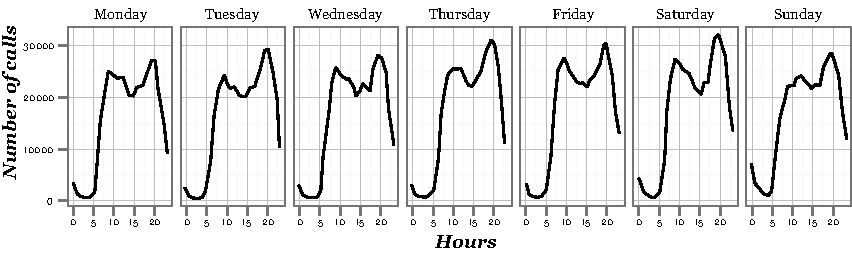
\includegraphics[scale =1.1] {results/images/calls_number.pdf}
\caption{Total amount of calls grouped by Week days}
\label{fig:count_calls}
\end{center}
\end{figure}



There are two peaks, $p_1$, from 7:00 am to 9:00 am, and another one, $p_2$, from 6:00 pm to 8:00 pm. As can be seen, the 'morning-peak' is lower than the 'evening-peak'. Moreover, both peaks reach their maximum value at the end of their corresponding time zone, i.e., $p_1$ at 9:30 am and $p_2$ at 7:30 pm. Note how the amount of calls increases linearly since 5 am and how it decreases linearly too since 8:00 pm. Another remarked feature is the existence of a central valley between $p_1$ and $p_2$, that is, from 9:00 am to 6:00 pm. This 'peak-valley-peak' pattern is shown for all days in the week, so that we can assume people have the same behaviour (at least, according to our target datasets).
\\
\\
Let's extract some ideas from the previous chart, focusing on what commuters could be probably doing (as we will see shortly, most of the phone calls belong to 'dynamic users'): they get up early in the morning and start to perform more and more phone calls from their handsets until $p1_$; next, the amount of phone calls decreases a bit, keeping itself more or less balanced (workhours, lunch) until the beginning of $p2_$; later, they people leave the office and plan the rest of the day (errands, leisure...), what is reflected on a marked rise in the amount of phone calls.
\\
\\
Since it is really complicated to measure the displacements of the people (antenna locations instead of users locations, missing antena identifiers...), what will be analyzed is the amount of callers who are really commuters, that is, dynamic users. This one will be the essential magnitude of our research, leading us to figure out the Commuting Dynamics key-features for different regions and times. Eventually, all conclusions deduced from the G/T Model (charts, formulae...) will be ultimately tested with the final GIS visualization as the main core of the work. In this last phase, geographical displacements are estimated so that they can be plotted in a dynamic and interactive map which makes easier to detect peaks, trends...
\\
\\


\begin{figure}[h]
\begin{center}
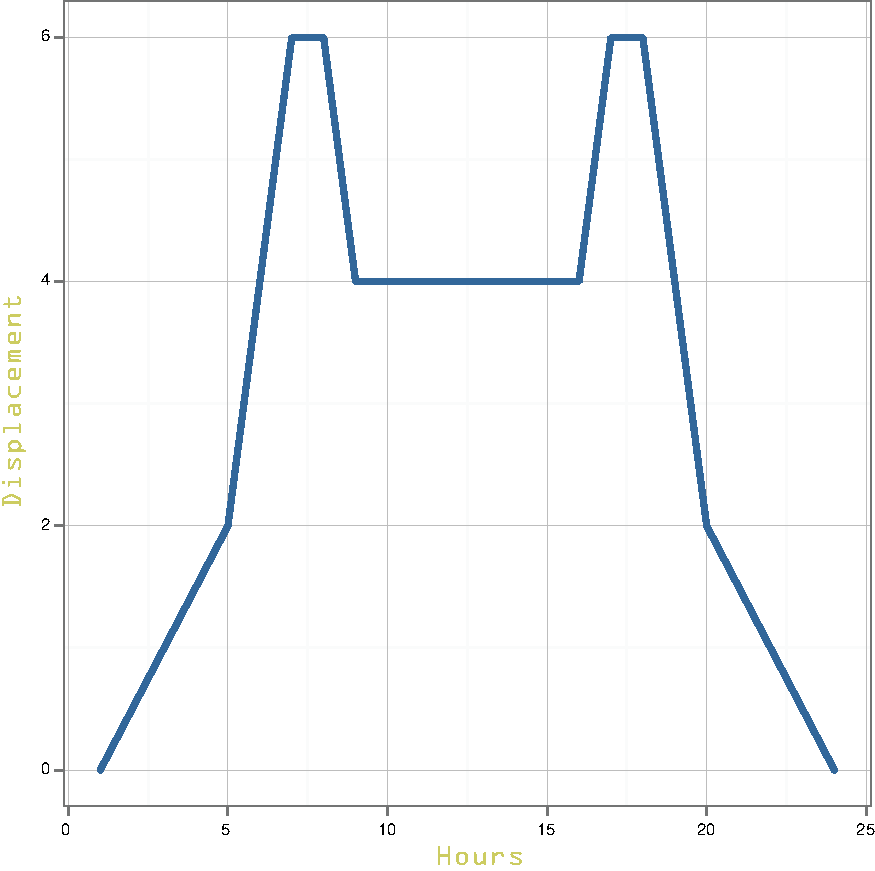
\includegraphics[scale =0.5] {results/images/common_commuting_model.pdf}
\caption{Theoretical Commuting Model}
\label{fig:commuting}
\end{center}
\end{figure}

With this new chart, it is the ratio between commuters and all users what it is being emphasized. During a particular day (24h), there is no need to know if a concrete displacement is or not longer than other, no, what it is being highlighted here is the movement detection itself, for 1h windows which groups all users calling within it. The colour of the chart shows how many users are really commuters.
\\
\\
Datasets have been processed according to the proposed G/T Model, filtering non-commuters when commuters tracks have been calculated. Here below, seven charts display Commuting Dynamics for each week-day.
As the results shows, the is not correlation between the number of dynamic users and the maximum displacement peaks, actually, at the same time the number of dynamic users are growing, the central valley an the two maximum commuting peaks are always presented in the sample.
\\
\\
These seven charts below shows a fitter correlation with the theoretical commuting model proposed in this paper (Figure ~\ref{fig:commuting}), showing two high peaks and a lower central valley. However more qualitative data is neccesary to figure out the performance of the first high peak, because is not related with the number of dynamic user, therefore a first approach can be applied to say that few dynamic users (in comparision with the mean) travel long distances in this first peak, specially in  the first uphill to the first peak. This is a common pattern figure out for the proposed model. However, because there are people that start his travel from a far distances early in the morning since the main people lives near the work places and travel less distances than the first one.  
\\
\\
 {\color{red} falta cruzar lo que se acaba de decir con las visualizaciones del kernel density, y listo more or less}


\begin{figure}[h]
\begin{center}
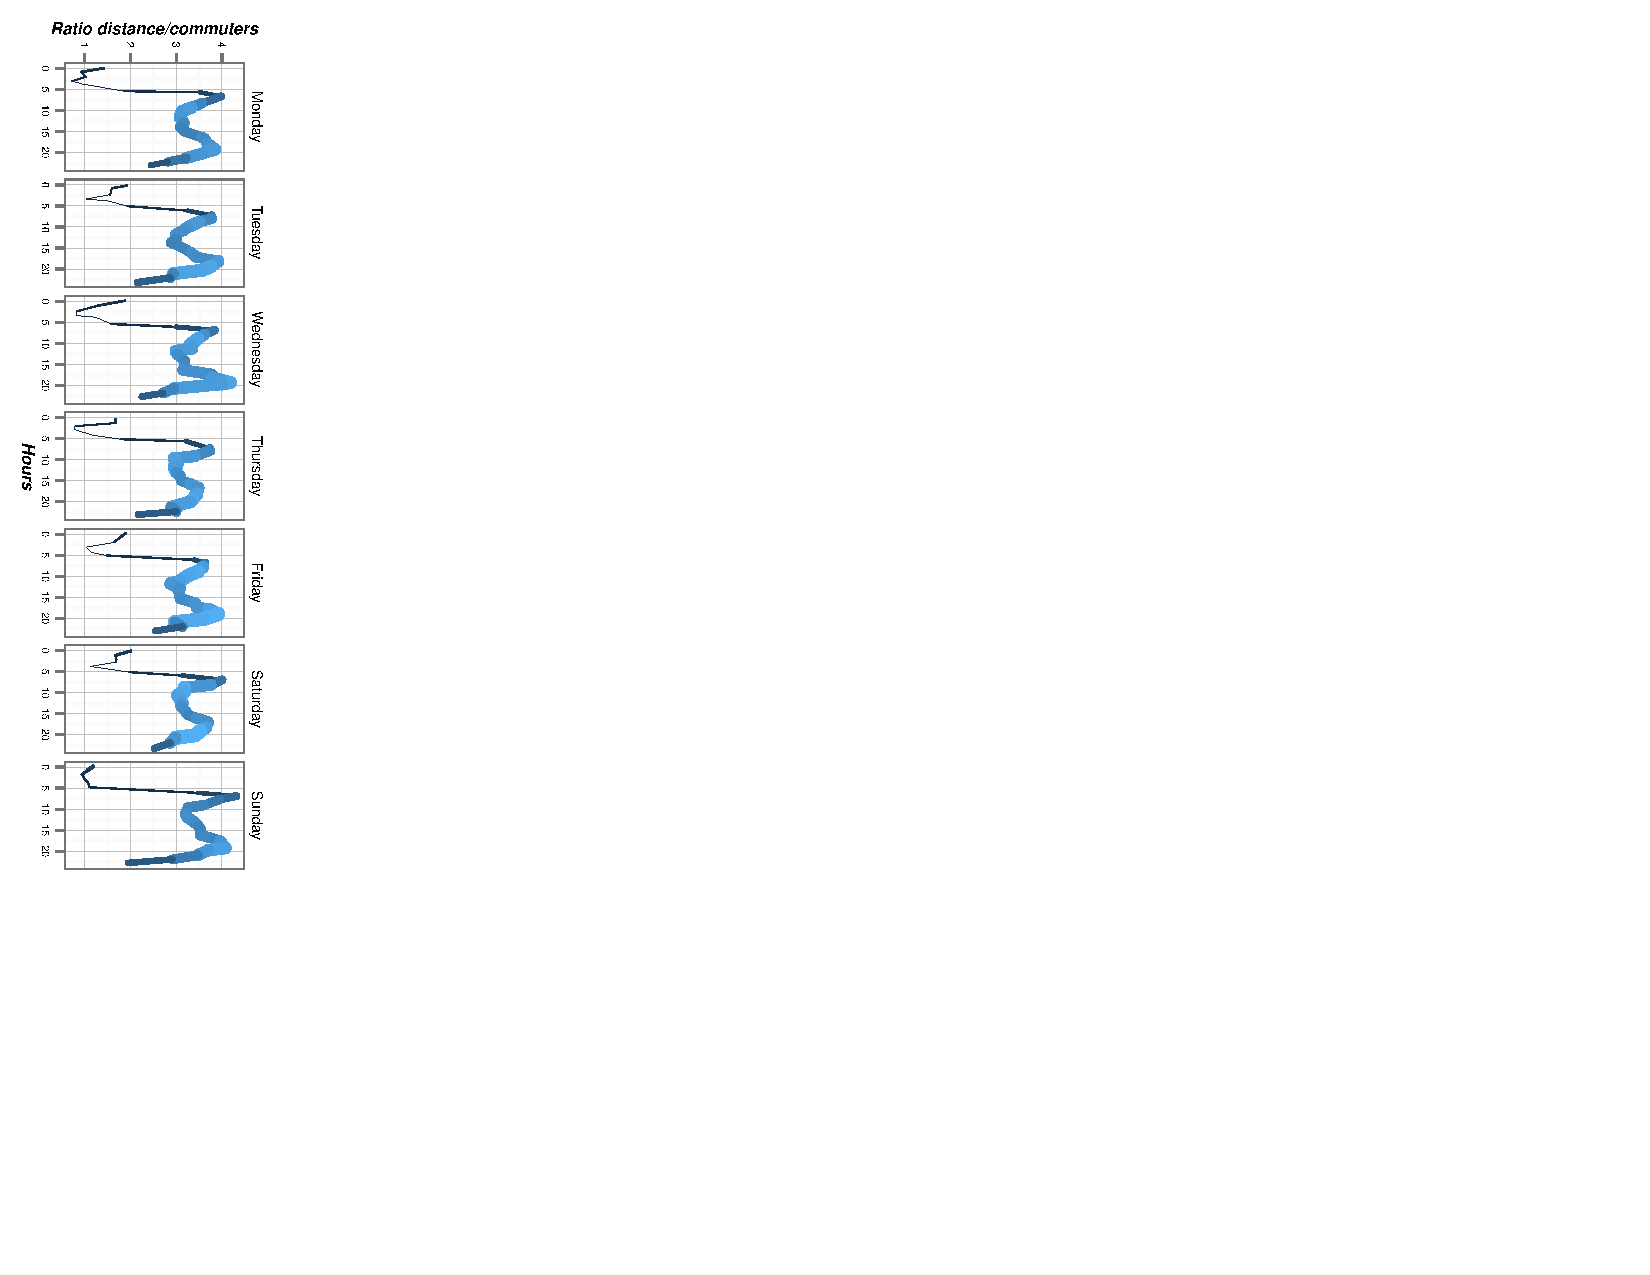
\includegraphics[scale = 1.0] {results/images/commuting_results.pdf}
\caption{Dynamic users displacements}
\label{fig:dynamic_displacements}
\end{center}
\end{figure}
